\section{Условный экстремум. Метод множителей Лагранжа}
Зачастую нас интересуют не локальные, а глобальные экстремумы.
Возникает логичный вопрос, как их искать?
Казалось бы, что достаточно найти все стационарные точки и сравнить значние в них.
Тогда самое большое/маленькое и будет глобальным максимумом/минимумом.
Но заметим, что если мы рассматриваем функцию на компакте, то мы обязаны рассмотреть ее и на границе, но стационарные точки определяются как внутренние.
То есть вдруг окажется так, что максимум/минимум лежит на границе?
Поэтому надо научиться справляться с точками на границе.

Иногда бывает также полезно искать экстремумы у функции, заданной на какой-то поверхности.
Например, функция температуры на планете задана на сфере, а вовсе не в $\R^3$.

Чтобы понять, как нам все это искать, введем определение условного экстремума.

\begin{conj}
    Пусть у нас есть:
    \begin{gather*}
        f: D \subset \R^{n+m} \to \R, \Phi: D \to \R^m, a \in D \text{ и } \Phi(a) = 0
    \end{gather*}
    Если существует $U$ -- окр-ть точки $a$, т.ч $\forall x \in U \cap D$ и $\Phi(x) = 0$, будет $f(x) \leqslant f(a)$, то $a$ -- \textbf{нестрогий условный максимум} при условии связи $\Phi = 0$.
    Точно также можно определить строгий максимум и аналогично минимум.
\end{conj}

Разберем это на примере.
У нас есть функция $f(x, y) = x^2 + y^2$ (оранжевый график).
Зададим функцию $\Phi(x, y) = x - 20$.
Точки, удовлетворяющие уравнению $\Phi = 0$ и лежащие на графике функции, будут образовывать зеленую кривую. 
Тогда точка $(20, 0, 400)$ будет строгим условным минимумом при условии связи $\Phi = 0$.

\begin{center}
    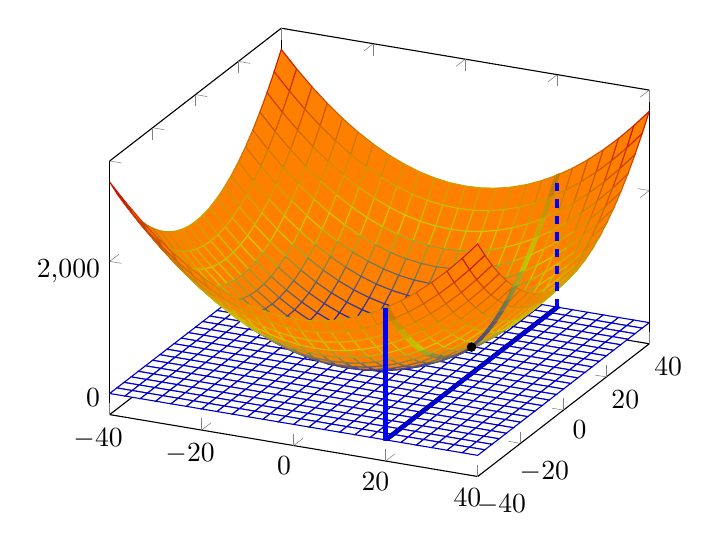
\begin{tikzpicture}
        \begin{axis} 
            \addplot3 [
                surf,
                white,
                shader=faceted,
                domain =-40:40,
                y domain=-40:40
                ] {0};

            \addplot3 [
                surf,
                orange,
                shader=faceted,
                samples=25,
                domain =-40:40,
                y domain=-40:40
                ] {x^2+y^2};

                \addplot3 [
                surf,
                black,
                shader=faceted,
                domain =19.5:20.5,
                y domain=-40:40
                ] {x^2+y^2};

                \addplot3 [
                surf,
                black,
                shader=faceted,
                domain =19.5:20.5,
                y domain=-40:40
                ] {0};

                \draw[blue, ultra thick] (axis cs:20, -40, 0) -- (axis cs:20, -40, 2000);

                \draw[blue, ultra thick, dashed] (axis cs:20, 40, 0) -- (axis cs:20, 40, 2000);
                
                \filldraw[black] (axis cs:20,0,400) circle(1.5pt);
    
        \end{axis}
    \end{tikzpicture}
\end{center}


Теперь нас интересует способ найти какие-то необходимые условия на условные экстремумы.
Для этого существует метод неопределенных множителей Лагранжа.

\vspace*{5mm}

\textbf{Метод множителей Лагранжа.} 

Пусть $f: D \subset \R^{n+m} \to \R$ непрерывно дифференцируема, $ \Phi: D \to \R^m$ непрерывно дифференцируема, $a \in \Int D$.
Тогда если $a$ точка условного экстремума при условии связи $\Phi = 0$, то $\nabla f, \nabla \Phi_1, \nabla \Phi_2, \dots, \nabla \Phi_m$ в точке $a$ линейно зависимы.

\notice \begin{enumerate}
    \item Если $\nabla \Phi_1, \nabla \Phi_2, \dots, \nabla \Phi_m$ линейно зависимы, то это случай не интересный, ведь тогда любая точка $a$, удовлетворяющая условию связи, будет точкой условного экстремума. 
    \item Если $\nabla \Phi_1, \nabla \Phi_2, \dots, \nabla \Phi_m$ линейно независимы, то существуют $\lambda_1, \dots, \lambda_m \in \R$, т.ч. $\nabla f = \lambda_1 \nabla \Phi_1 + \dots + \lambda_m \nabla \Phi_m$.
    Это просто по определению: у нас была ЛНС, добавили 1 вектор, стала ЛЗС $\Rightarrow$ можем выразить в виде линейной комбинации.
    \item Что означает линейная независимость $\nabla \Phi_1, \nabla \Phi_2, \dots, \nabla \Phi_m$?
    Вспоним, что эти градиенты -- строки матрицы Якоби $\Phi$ в точке $a$ (у этой матрицы $m$ строк и $n+m$ столбцов).
    Таким обоазом, это означает, что $\rk \Phi'(a)$ максимален, то есть равен $m$.
    
    Мы также можем упростить запись во втором пукнте, если представим лямбды как вектор-строку: $\lambda = (\lambda_1, \dots, \lambda_m) \Longrightarrow \nabla f = \lambda_1 \nabla \Phi_1 + \dots + \lambda_m \nabla \Phi_m = \lambda \Phi'(a)$.
\end{enumerate}

\begin{proof}
    Ранг $\Phi'(a) = m$ и надо доказать, что $f'(a) = \lambda \Phi'(a)$ для некоторого $\lambda \in \R^m$.
    В условии говорилось про $\nabla f$, но $f$ действует в $\R$, поэтому $\nabla f$ в точке $a$ равно $f'(a)$.

    Считаем, что минор $\Phi'(a)$ по последним $m$ координатам $\neq 0$.
    Мы всегда можем этого добиться, попереставляв их, ведь $\rk \Phi'(a) = m$.
    Будем обозначать $a = (b, c)$, где $c$ как раз и будет последними $m$ координатами.
    Так как там минор $\neq 0$, мы можем применить теорему о неявно заданной функции.
    Согласно ней $\exists W$ окр-ть точки $b$ и непрерывно дифференцируемая функция $g: W \to \R^m$, т.ч. $g(b) = c$ и $\Phi(x, g(x)) = 0 \;\; \forall x \in W$.
    \textit{Вообще у нас тут поменялся порядок по сравнению с оригинальной формулировкой теоремы, но это и логично, потому что минор у нас ненулевой уже по последним координатам, а не по первым.}

    Введем \begin{gather*}
        h(x): W \to \R^m \\ h(x) = f(x, g(x))
    \end{gather*} 
    Заметим, что $b$ будет экстремумом для $h$, так как при $x$ близком к $b$ у нас $g(x)$ будет близко к $c$, таким образом $(x, g(x))$ будет близко к $a$. А это условный экстремум по условию.

    В силу необходимого условия экстремума получаем, что $h'(b) = 0$.
    Давайте посчитаем эту производную. 
    Для этого разобьем матрицу из частичных производных $f(a)$ на 2: $f'_x(a)$ -- матрица из частных производных по первым координатам, $f'_y(a)$ -- матрица из частных производных по последним координатам.
    Тогда: \[ h'(b) = f'_x(a) + f'_y(a) \cdot g'(b) = 0 \]
    Вспоним, что $\Phi(x, g(x)) \equiv 0$ (тут 0 как функция), и точка $b$ лежит в области определения. 
    Производная 0 равна 0, поэтому: \[ \Phi'(b, g(b)) = \Phi_x'(a) + \Phi_y'(a)\cdot g'(b) = 0  \]
    Вычтем из $h'(b)$ последнее выражение, домноженное на произвольное $\lambda \in \R^m$ : \[ h'(b) - \lambda \Phi'(b, g(b)) = (f'_x(a) - \lambda \Phi_x'(a)) + (f'_y(a) - \lambda \Phi_y'(a))\cdot g'(b) = 0  \]
    Осталось правильным образом выбрать $\lambda$. 
    Давайте выберем ее так, что $f'_y(a) - \lambda \Phi_y'(a) = 0$. 
    Мы так можем сделать, потому что  минор $\Phi'(a)$ по последним координатам $\neq 0$, а $y$ это как раз и есть последние координаты.
    Поэтому уравнение $f'_y(a) - \lambda \Phi_y'(a) = 0$ будет разрешимо относительно $\lambda$.

    Мы занулили второе слагаемое, поэтому обязано занулиться и первое: $f'_x(a) - \lambda \Phi_x'(a) = 0$.
    Если объединить эти результаты, то получится, что: \[ f'(a) = \lambda \Phi'(a) \]
    Что и требовалось доказать.
\end{proof}

\vspace*{5mm}

А как все-таки на практике искать такие $a$?
В уравнении $f'(a) = \lambda \Phi'(a)$ у нас $2m + n$ неизвестных: $n + m$ координат точки $a$ и $m$ координат $\lambda$.
Посмотрим на число уравнений. 
Уравнение $f'(a) = \lambda \Phi'(a)$ распадается на $n + m$ штук (по каждой координате $a$).
Также точка $a$ обязана удовлетворять уравнению $\Phi(a) = 0$, что дает еще $m$ уравнений.
Таким образом, чтобы найти $a$ и $\lambda$ надо решить систему из $2m + n$ уравнений от такого же количества неизвестных. 
 
\vspace*{5mm}

\begin{conj}
    Функция Лагранжа -- функция, которая в наших предыдущих обозначениях равна $f - \lambda \Phi$.
    Таким образом, чтобы найти условные экстремумы, надо искать точки, где производная функции Лагранжа нулится.
\end{conj}
